\documentclass[letter, 10pts]{article}
\usepackage[monocolor]{../math232/ahsansabit}
\usepackage[]{float}
\usepackage{tikz}
\usepackage{tikz-3dplot}
\usepackage[outline]{contour} % glow around text
\usepackage{xcolor}
\usepackage{pdfpages}
\usepackage{physics}
\usepackage{multicol}
\title{Quantum Mechanics : : Homework 01}
\author{Ahmed Saad Sabit, Rice University}
\date{\today}
\newcommand{\hb}{\hbar}
\newcommand{\U}{\uparrow}
\newcommand{\D}{\downarrow}
\usepackage[]{braket}
\begin{document}
\maketitle

\section*{Problem 1} 
\hrule 
The first statement in the problem in mathematical sense is 
\[
\braket{x | \psi} = 
\begin{cases} 
	\psi(x) = c  & - a < x  < a \\  
	\psi(x) = 0 & \text{elsewhere} 
\end{cases}
\] 
The corresponding wave function in momentum representation is 
\[
\psi(p) = \braket{p | \psi}
=
\braket{p | \hat{I} | \psi} 
= \bra{p}  
\int_{-\infty}^{\infty}  \mathrm{d} x \,   
\ket{x} \braket{x | \psi}
\] 
Which gives us 
\[
\psi(p) = \int_{-\infty}^{\infty} 
\mathrm{d} x \, 
\braket{p | x} \psi(x) 
=
\int_{-\infty}^{\infty} 
\mathrm{d} x \, 
\frac{\psi(x)}{\sqrt{2 \pi \hb} } e^{ - i p x / \hb}
\]
This can be computed using what we have 
\begin{align*}
	\psi(p) &= \frac{1}{\sqrt {2 \pi \hb} } 
\int_{-\infty}^{\infty} \psi(x) e^{ - i p x / \hb} \, \mathrm{d} x \\ 
&= \frac{1}{\sqrt{2 \pi \hb} } \int_{-a}^{a}  c e^{ - i p x / \hb } \, \mathrm{d} x  \\ 
&= \frac{1}{\sqrt{2 \pi \hb} } c 
\left[
\frac{1}{- i p / \hb} (e^{- i p a / \hb} - e^{i p a / \hb})	
\right]\\
&= \frac{c}{\sqrt{2 \pi \hb} } 
\left[
\frac{\hb}{i p } (e^{ i p a / \hb} - e^{- i p a / \hb})	
\right]\\
&= \frac{2c \hb}{p \sqrt{2 \pi \hb} } 
\left[
\frac{1}{2i } (e^{ i p a / \hb} - e^{- i p a / \hb})	
\right]\\
&= \frac{2c \hb}{p \sqrt{2 \pi \hb} } 
\sin(a p / \hb ) \\
&= 
\sqrt{\frac{2\hb c^2}{\pi p^2}} 
\sin(a p / \hb ) \\
\end{align*}

Normalization gives us a clue what could be $\psi(x)$ which is 
\[
\int \psi(x)^2 \mathrm{d} x = c^2 2 a = 1 \to  c = \sqrt{\frac{1}{2 a}} 
\] 


Hence
\[
\psi(p) = \sqrt{ \frac{\hb }{\pi a p^2}}  \sin (a p / \hb)
\] 
\begin{figure}[H]
	\centering
	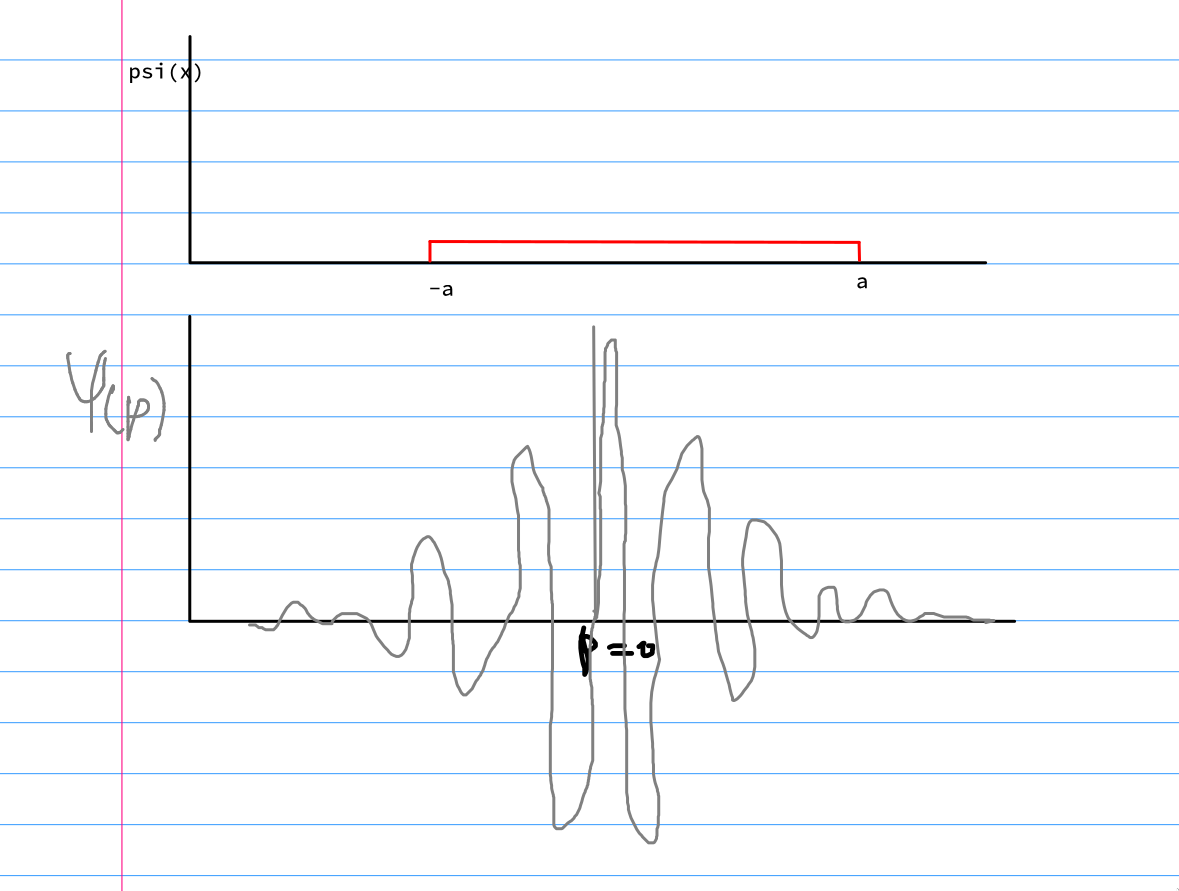
\includegraphics[width=0.8\textwidth]{./ss/1/1.png}
	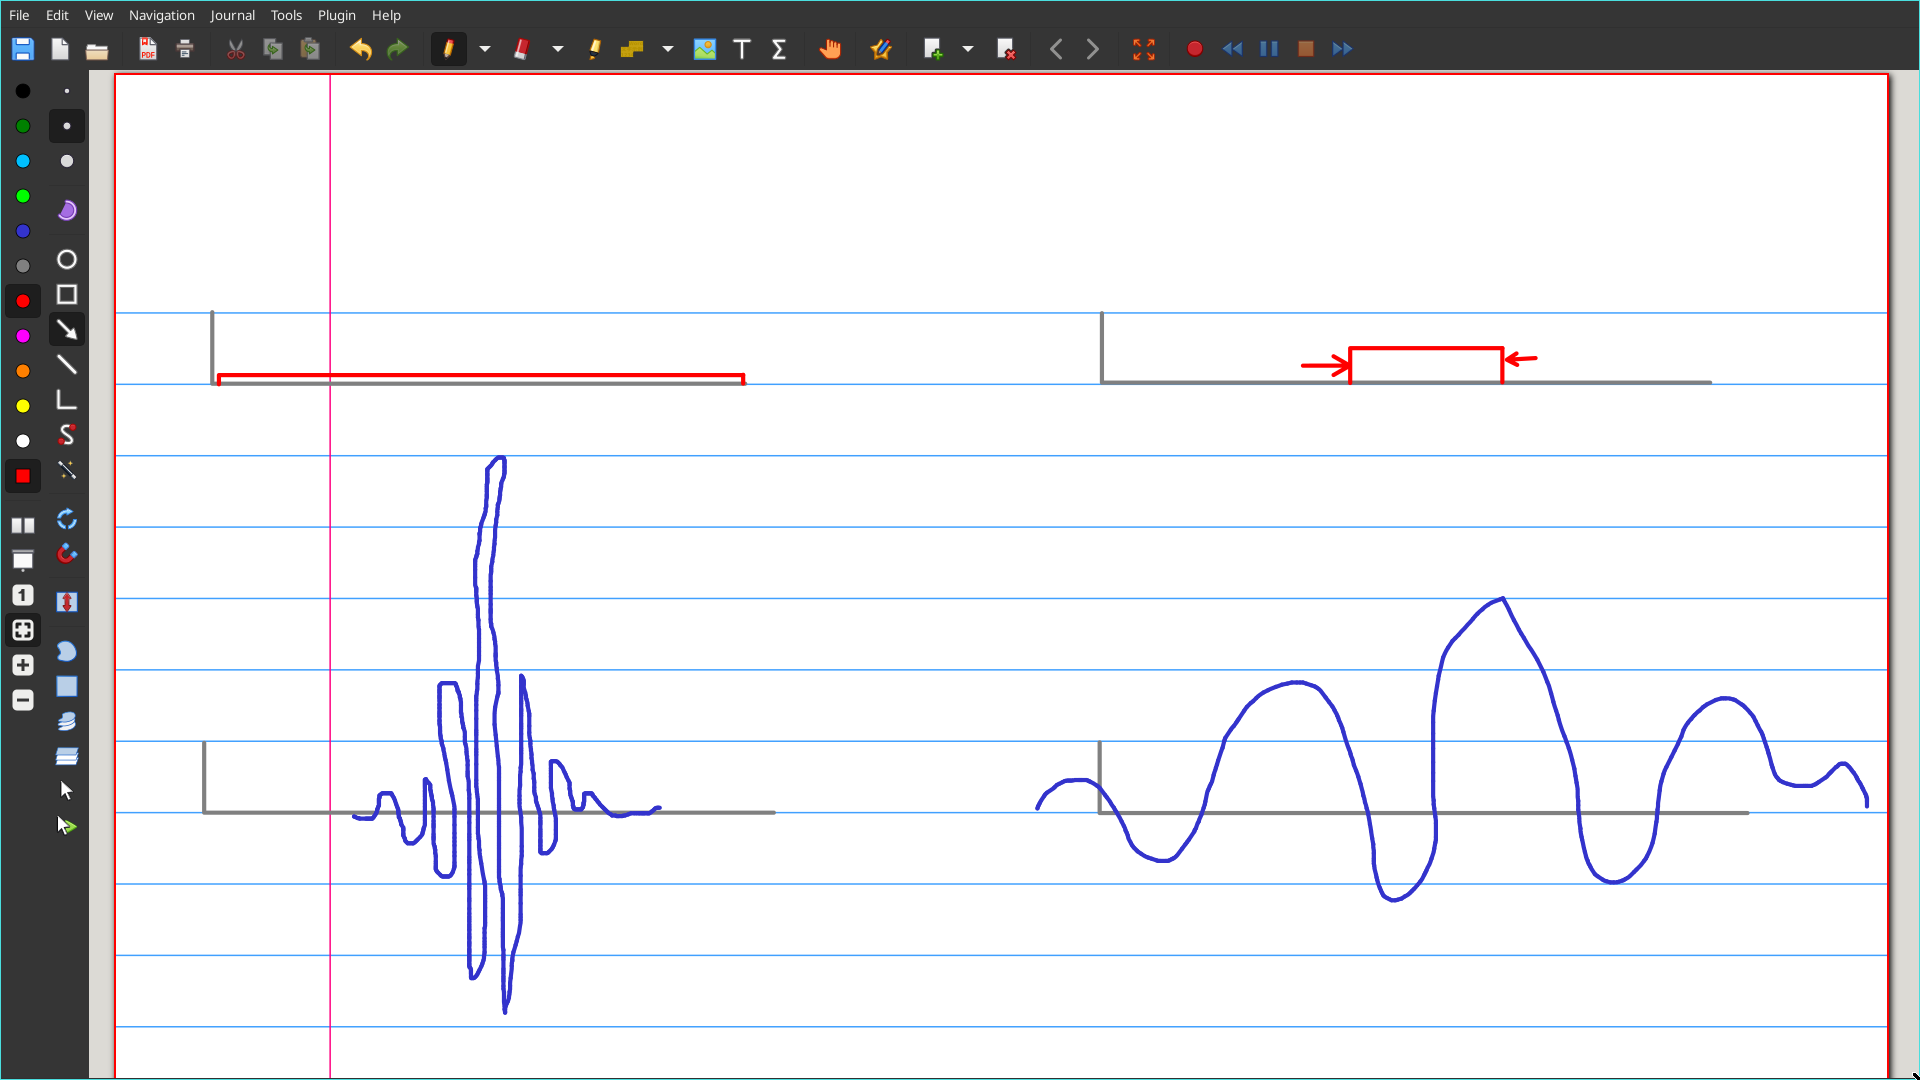
\includegraphics[width=0.8\textwidth]{./ss/1/2.png}
	\caption{For large and small $a$}
	\label{fig:-ss-1-1-p}
\end{figure}
\textbf{For $a \to  0$:} In this case we have an extremely high amount of localization. This will make $p$ very large because of uncertainty. Evidently from what we say from normalization of $\psi(x)$ the wavefunction will apparently look like a spike centered at origin.


\textbf{For $a \to \infty$} This will localize $p$ in a sense by making the error small, where we do have a dirac delta-like spike centered in origin. 





\newpage
\section*{Problem 2} 
\hrule 

\subsection*{(a)} 
Projection operator will satisfy the relation $\Lambda^2 = \Lambda$, hence computing $\Lambda^2$
\begin{align*}
\Lambda^2 &= 
\frac{1}{2} (I + P)
\frac{1}{2} (I + P)
\\
&= 
\frac{1}{4} (I^2 + IP + P I + P ^2)
\\
&= 
\frac{1}{4}
(I + 2 P + I)
\\
&= 
\frac{1}{4}
(2I + 2 P )
\\
&= \frac{1}{2} ( I + P ) \\ 
&= \Lambda \\
\end{align*}
We find that $\Lambda^2 = \Lambda$ hence $\Lambda$ is a projection operator (proved). 




\subsection*{(b)} 
Similar to the previous analysis we did 
\begin{align*}
\overline{\Lambda} ^2 &= 
(I - \Lambda )(I - \Lambda )\\
&= I - I \Lambda  - \Lambda I + \Lambda^2 \\
&= I - 2 \Lambda + \Lambda \\ 
&= I - \Lambda \\ 
&= \overline{ \Lambda} \\
\end{align*}
Hence proving $\overline{\Lambda}$ is also a projection operator. Now, if $\overline{\Lambda}$ and $\Lambda$ are orthogonal, they will satisfy the relation $\hat{A} \hat{A}_\perp = \hat{A}_\perp \hat{A} = 0$ 

\begin{minipage}{0.5\textwidth}
\begin{align*}
\overline{\Lambda} \Lambda &= 
(I - \Lambda) \Lambda 
\\
&= I \Lambda - \Lambda^2  \\
&= \Lambda - \Lambda \\ 
&= 0 \\
\end{align*}
\end{minipage}
\hfill
\begin{minipage}{0.5\textwidth}
\begin{align*} \Lambda
	\overline{\Lambda} &= \Lambda ( I - \Lambda) \\
	&= \Lambda I - \Lambda ^2 \\
	&= \Lambda - \Lambda \\ 
	&= 0 \\
\end{align*}
\end{minipage}
Hence both $\Lambda$ and $\overline{\Lambda}$ are orthogonal projection operators (proved).



\subsection*{(c)} 
Let $T$ be a non trivial projection operator. This means this $T$ will satisfy $T^2 = T$. Then 
\[
T^{-1} T = I 
\]
Introduce a $T$ on the right
\[
	(T^{-1} T) T = T 
\]
This yields
\[
T^{-1} T^2 = T 
\]
Now, by using the rule of a non trivial projection operator 
\[
T^{-1} T = T 
\] 
This shows (after comparing with the first equation $T^{-1} T = I$) that $T = I$. This is a trivial projection operator, which leaves the vector as it was. So $T$ cannot have an inverse otherwise it's just a trivial projection (the identity operator). 





\section*{Problem 03} 
\hrule 
\subsection*{(a)} 

Let's create the equation in the problem first to motivate the solution. The central potential Hamiltonian is given by 
\[
H = \frac{\vec{p}^2}{2m} + V(r)
\]
The eigenequation for this is 
\[
H \ket{E,l,m} = E \ket{E,l,m}
\] 
Now we know the radial equation (Sakurai 3.230) that
\[
\frac{1}{2m} \bra{\vec{r}} \vec{p}^2 \ket{\Psi} = 
- \left(\frac{\hb^2}{2m}\right) \nabla ^2 \braket{\vec{r} | \Psi} = 
- \left(\frac{\hb^2}{2m}\right) 
\left(
\frac{\partial ^2}{\partial r^2} \braket{\vec{r} | \Psi} + 
\frac{2}{r} \frac{\partial}{\partial r} \braket{\vec{r} | \Psi} - 
\frac{1}{\hb^2 r^2} \braket{\vec{r} | \vec{L}^2 | \Psi }
\right)
\] 
Using this above equation with $\Psi = R_{El} Y_{l,m}$ and $\vec{L}^2 \ket{E,l,m} = l(l+1) \hb^2 \ket{E,l,m} $ we get 
\[
\left[
- \frac{\hb^2}{2m } \frac{\mathrm{d} }{\mathrm{d} r} 
\left(r^2 \frac{\mathrm{d} }{\mathrm{d} r}\right)
+ 
\frac{l(l+1)\hb^2}{2mr^2} + V(r)
\right] R_{El}(r) = E R_{El}(r)
\] 
Let us make the following substitution as instructed in the problem $R_{El}(r)  = u(r) / r$ then we get the following equation
\[
	- \frac{\hb^2}{2m } \frac{\mathrm{d} ^2}{\mathrm{d} r^2} u_{El} + 
\left(
\frac{l(l+1) \hb^2}{2 m r^2} + V(r) 
\right) u_{El}(r) = Eu_{El}(r)
\] 
With some basic algebraic manipulation
\[
	\frac{\mathrm{d} ^2}{\mathrm{d} r^2} u_{El} - \frac{l(l+1)}{r^2} u_{El} +k^2 u_{El} - \frac{2mV(r)}{\hb^2} u_{El}(r) = 0 
\] 

\[
	\frac{\mathrm{d} ^2}{\mathrm{d} r^2} u_{El}+k^2 u_{El} -  \left( \frac{l(l+1)}{r^2}  + \frac{2mV(r)}{\hb^2}\right) u_{El}(r) = 0 
\] 
What we get for effective potential is 
\[
	\tilde{V}(r) = \frac{2m}{\hb^2} V(r) + \frac{l(l+1)}{r^2}
\] 



\subsection*{(b)} 
According to the question at $r \to  \infty$ we will end up getting
\[
	\tilde{V}(r) = \frac{2m}{\hb^2} V(r) + \frac{l(l+1)}{r^2} \to  0
\]
Which makes sense because if $V(r)$ goes to zero faster than $1 / r$, then it's also obvious that $\frac{1}{ r^2} l (l+1)$ will also go faster than $1 / r$. 
Hence, 
\[
\frac{\mathrm{d} ^2}{\mathrm{d} r^2} u + k^2 u = 0 
\]
Because $E = \frac{\hb ^2}{2 m} k^2$ hence positive energy corresponds to positive $k$ for which we get a solution of the form $u \propto e^{i k r}$ which qualitatively means that the particle is unbounded. And that is true because $E > 0$. For unbounded states $E < 0$ we get
\[
\frac{\mathrm{d} ^2}{\mathrm{d} r^2} u = k^2 u 
\] 
This means $u \propto e^{-k r}$ which is a bound state solution that says that as we go far away from the ``nucleus" the more unlikely it is to find the particle. This is true given the bounded condition. 


\subsection*{(c)}  Now in our problem $V(r)$ goes to zero like $\frac{1}{r}$. And $1 / r^2$ definitely goes to zero faster than $ 1 / r$ so again we have the exact same case as (b). 

Our answers are verified because every Hydrogenic wavefunctions mentioned in the Problem (referenced to Townsend) has an $e^{-r}$ term that exactly agrees to our findings in $E < 0$ bound states, leaving no room of confusion that what we have is qualitatively valid. 



















\section*{Problem 04} 
\hrule 
\subsection*{(a)} 
\begin{align*}
	[p_i , r^2] &= \left[p_i , \sum_{j}^{3} x_j x_j\right] \\
		    &= [p_i, x_j x_j]  \\
		    &= p_i x_j x_j - x_j x_j p_i   \\
		    &= p_i x_j x_j - x_j p_i x_j + x_j p_i x_j - x_j x_j p_i \\
		    &= [p_i, x_j] x_j + x_j [p_i, x_j]  \\
		    &= - i \hb \delta_{ij} \cdot  x_j - x_j \cdot  (i \hb \delta_{ij}) \\
		    &= -2i \hb x_i  \\
\end{align*}


\subsection*{(b)} 
We will reuse some mathematical trick steps from (a). 
\begin{align*}
	[r^2, p^2] &= \left[
		\sum_{i}^{3} x_i x_i, 
		\sum_{j}^{3} p_j p_j
	\right]\\
		   &= [x_i x_i , p_j p_j] 
		  \\
		   &=[x_i x_i, p_j]p_j + p_j[x_i x_i, p_j]  \\
		   &=-[p_j,x_i x_i]p_j - p_j[p_j,x_i x_i]  \\
		   &= -[p_j, x_i]x_i p_j - x_i[p_j, x_i]p_j
		   -p_j [p_j, x_i] x_i - p_j x_i[p_j,x_i]\\
		   &= (i \hb \delta_{ij}) x_i p_j + 
		   x_i (i \hb \delta_{ij}) p_j + 
		   p_j (i \hb \delta_{ij}) x_i 
		   + 
		   p_j x_i (i \hb \delta_{ij})\\
		   &=2 i\hb (x_i p_i + p_i x_i) \\
		   &= 2i\hb (x_i p_i + x_i p_i - i \hb ) \\
		   &= 4 i \hb x_i p_i + 2 \hb^2 \\
\end{align*}








\end{document}
